%%=============================================================================
%% Methodologie
%%=============================================================================

\chapter{Methodologie}
\label{ch:methodologie}

%% TODO: Hoe ben je te werk gegaan? Verdeel je onderzoek in grote fasen, en
%% licht in elke fase toe welke stappen je gevolgd hebt. Verantwoord waarom je
%% op deze manier te werk gegaan bent. Je moet kunnen aantonen dat je de best
%% mogelijke manier toegepast hebt om een antwoord te vinden op de
%% onderzoeksvraag.
Dit hoofdstuk beschrijft hoe men het best te werk gaat voor de opzet van een eenvoudig, kleinschalig blockchain gebaseerd stemsysteem. Het volledige proces wordt hier weergegeven in de vorm van een praktische handleiding,  voornamelijk bedoeld voor ontwikkelaars die niet vertrouwd zijn met het ontwikkelen van Dapps. Gezien de vrij technische aard van deze handleiding wordt er wel van uit gegaan dat de lezer enige vorm van algemene voorkennis heeft op het vlak van programmatie. Kennis van Solidity wordt niet verondersteld. De implementatie die hier wordt besproken gebeurt op basis van de verschillende technieken die werden toegelicht in het vorig hoofdstuk. Er wordt gekozen voor het Ethereum blockchain platform als ontwikkelomgeving, deze keuze gebeurt op basis van sectie \ref{sec:ethereum-en-smart-contracts} van het vorige hoofdstuk. In dit hoofdstuk bieden we verder antwoord op de onderzoeksvragen \textit{wat de praktikaliteit van een blockchain gebaseerd stemsysteem is}, \textit{hoe haalbaar een blockchain gebaseerd stemsysteem is} en tenslotte ook \textit{of er sprake van een onoverkomelijk schaalbaarheidsprobleem}.

\section{Benodigdheden}
\label{sec:benodigdheden}
De volgende zaken dienen geïnstalleerd te worden voor men van start kan gaan met het implementeren van een gedecentraliseerde Ethereum blockchain applicatie:
\begin{itemize}
	\item{Node.js}
	\item{npm}
	\item{Truffle}
	\item{Ganache}
	\item{Metamask}
\end{itemize}
Daarnaast heeft men ook nodig:
\begin{itemize}
	\item{Een IDE code-editor naar keuze met syntax ondersteuning voor Solidity}
	\item{Google Chrome}
\end{itemize}

\subsection{ node en npm}
Node.js is een veelgebruikte Runtime-omgeving waarmee Javascript op ieder platform uitgevoerd kan worden, zonder dat daar een browser voor nodig is. Npm is een pakketbeheerder voor Javascript code. Npm zit standaard in Node.js en is `s werelds grootste softwareregister. Open source-ontwikkelaars wereldwijd gebruiken het om pakketten te delen, veel organisaties gebruiken npm om ook hun privéontwikkeling te beheren (\ref{fig:nodejs}).\footnote{Verkregen en vertaald van https://docs.npmjs.com/about-npm/}

Eenmaal node\footnote{node met npm is verkrijgbaar via https://nodejs.org} en npm\footnote{npm is ook apart verkrijgbaar via https://www.npmjs.com/get-npm} geïnstalleerd zijn, verifieert men de installatie via het console-commando: 
\lstset{language=bash}
\begin{lstlisting}[numbers=none]
> node -v
\end{lstlisting}Bij correcte installatie geeft dit de huidige node versie terug, bijvoorbeeld \textit{v10.15.1}. 

\begin{figure}
	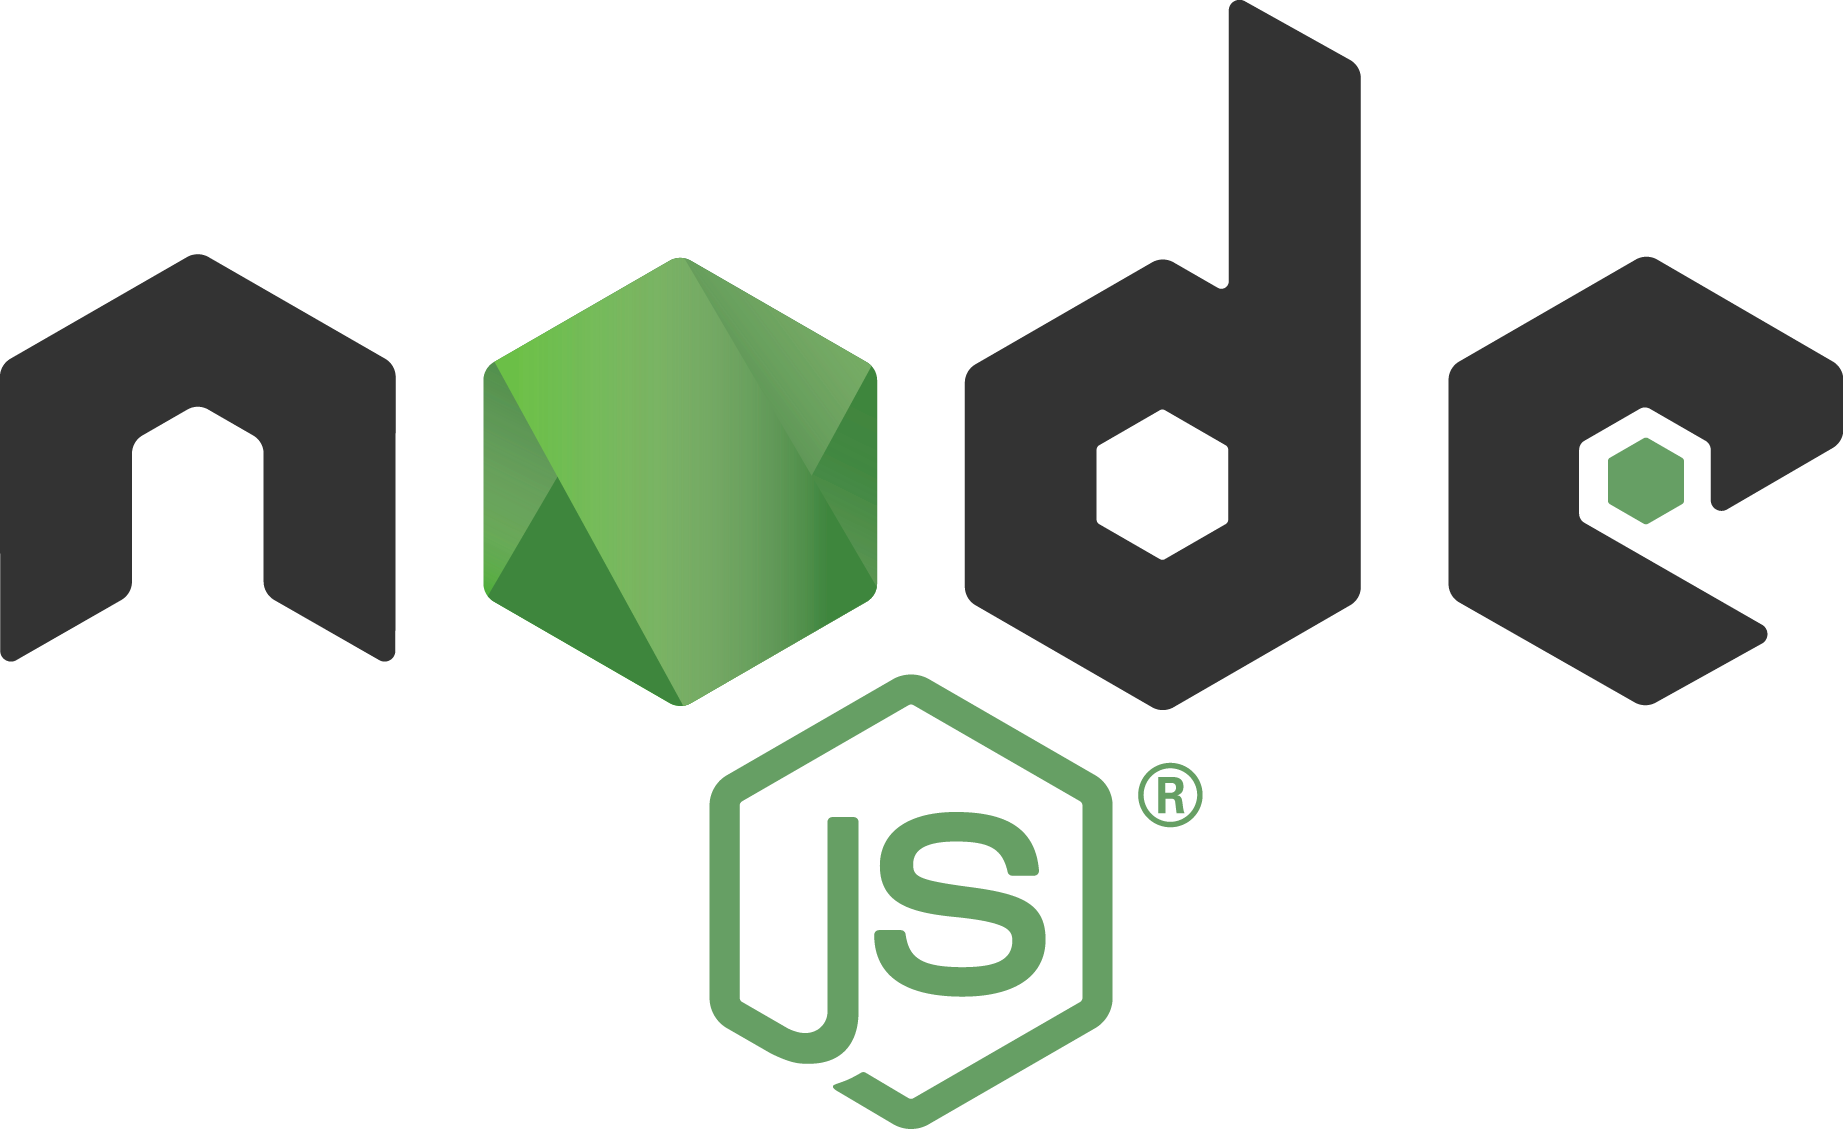
\includegraphics[width=\linewidth/2]{img/nodejs.png}
	
\includegraphics[width=\linewidth/2]{img/npm.png}
	\caption{De Node.js en npm logo's}
	\label{fig:nodejs}
\end{figure}

\subsection{Truffle}
Truffle is een ontwikkelomgeving, testframework en asset pipline, gericht op het versoepelen van het Ethereum ontwikkelproces. Het bevat ook verschillende code-templates die als basis kunnen worden gebruikt om gedecentraliseerde applicaties te ontwikkelen.

Truffle kan eenvoudig geïnstalleerd worden via npm (mits dit  voorgeïnstalleerd is) met het console-commando:
 \lstset{language=bash}
\begin{lstlisting}[numbers=none]
> npm install truffle
\end{lstlisting}
\subsection{Ganache}
Ganache\footnote{Ganache is verkrijgbaar via https://www.trufflesuite.com/ganache} is een applicatie die ontwikkelaars in staat stelt om een private Ethereum-blockchain op te zetten. We gebruiken deze blockchain gedurende de volledige ontwikkelperiode. Op deze manier kan men kosteloos smart-contracts ontwikkelen en testen. Indien men direct op de Ethereum hoofdketen ontwikkelt dan is immers er aan iedere transactie  een kost verbonden. Ganache biedt ons 10 externe accounts om te gebruiken tijdens het ontwikkelen. De accounts hebben adressen die corresponderen met adressen op een lokale Ethereum-blockchain. Elke account is vooraf geladen met 100 nep-ether.

\subsection{Metamask}
Metamask\footnote{Metamask is verkrijgbaar via https://metamask.io of via https://chrome.google.com/webstore} is een plugin voor Google Chrome die ontwikkelaars toelaat Ethereum dApps uit te voeren in de browser zonder zelf een node te moeten zijn in het netwerk, door Metamask te installeren hoeft men met andere woorden dus de volledige blockchain niet meer te downloaden.

\begin{figure}
	
\includegraphics[width=\linewidth]{img/metamask-truffle-ganache.png}
	\caption{Truffle, Metamask en Ganache logo's}
	\label{fig:metamask-truffle-ganache}
\end{figure}

\section{Implementatie Smart Contracts}

Eenmaal al de verschillende tools en plugins uit sectie \ref{sec:benodigdheden} geïnstalleerd zijn kan men aan het ontwikkelen van smart-contracts beginnen. In de volgende subsecties volgt de implementatie van een blockchain gebaseerd stemsysteem op basis van smart-contracts. We beginnen met een simpele implementatie, die niet self-tallying is. Vervolgens zullen we de nodige cryptografie toevoegen om een systeem gelijkaardig aan het Open Network Protocol van  \textcite{McCorry2017} te bekomen.

\subsection{Opzet}
Voor we beginnen met het ontwikkelen van onze smart-contracts moeten we eerst een ontwikkelomgeving opzetten. Voor een vlotte opstart maken we gebruik van één van de template projecten beschikbaar via truffle. Na te navigeren naar een gewenste directory, gebruikt men het console commando: 
 \lstset{language=bash}
\begin{lstlisting}[numbers=none]
> truffle unbox pet-shop
\end{lstlisting}

Dit creëert een nieuw project in de huidige directory, we openen het in een code-editor (in dit voorbeeld VS-code).

\subsection{Belang van testen}
Bij het ontwikkelen van dApps speelt testen nog  meer een cruciale rol  dan het bij de traditionele software ontwikkeling doet. Vermits het deployen van contracts op de blockchain verbonden is aan een gas prijs, is het bijzonder onwenselijk dat er bugs in de code sluipen die ervoor kunnen zorgen dat we moeten herdeployen. Functies die bugs bevatten en onverwacht gedrag vertonen kunnen erg kostelijk zijn voor gebruikers door de extra verwerkings-kosten die ze vergen. Doordat alles dat in de blockchain wordt bewaard immutable is, betekend het herdeployen van een smart-contract eigenlijk dat het huidige contract wordt vervangen door een nieuwe kopie, zowel de state als het adres van het oude contract gaan hierbij verloren. Dat is niet alleen bijzonder onpraktisch, het is ook brekend voor iedere front-end applicatie die aan de dApp verbonden is. 

Door smart-contracts grondig te testen kunnen we dergelijke situaties vermijden.

Er zijn verschillende methoden die men kan toepassen om een smart-contract te testen, standaard is om ze te schrijven in Solidity. Voor dit voorbeeld zullen we echter gebruik maken van Javascript. Via truffle kunnen we met behulp van Javascript de  interacties van gebruikers met onze smart-contracts gemakkelijk simuleren. Truffle bevat immers standaard Mocha\footnote{Apart verkrijgbaar via https://mochajs.org} (testframework) en Chai Assertion Library\footnote{Apart verkrijgbaar via https://www.chaijs.com}. Deze twee tools stellen ons instaat om onze smartcontracts te importeren binnenin Javascript-testen. 

 \lstset{language=JavaScriptSolidity} 
 \begin{lstlisting}[frame=single] 
 var Election = artifacts.require("./Election.sol");
 	
 contract("Election", function(accounts){
	var electionInstance;
	 
	it("Initializes two candidates", function() {
	 	return Election.deployed().then(function(instance){
	 		return instance.candidatesCounter();
	 	}).then(function(count){
	 		assert.equal(count,2);
	 	});
 	});
 	
	it("Initializes yes and no", function() {
 		return Election.deployed().then(function(instance){
 			electionInstance = instance;
 			return electionInstance.candidates(1);
 		}).then(function(candidate){
			assert.equal(
		 	candidate[0],1,"has the correct id: 1"
		 	);
			assert.equal(
			 	candidate[1],"Yes","has the correct value: `Yes'"
			);
			assert.equal(
			 	candidate[2],0,"has the correct amount of votes: 0"
			);
			return electionInstance.candidates(2);
 		}).then(function(candidate){
			assert.equal(
				candidate[0],2,"has the correct id: 2"
			);
			assert.equal(
				candidate[1],"No","has the correct value: `No'"
			);
			assert.equal(
				candidate[2],0,"has the correct amount of votes: 0"
			);
 		}); // End function
 	}); // End it()
}); // End contract
\end{lstlisting}

\lstset{language=JavaScriptSolidity} 
\begin{lstlisting}[frame=single] 
pragma solidity ^0.5.8;

contract Election {
	// Store candidate
	struct Candidate {
		uint id;
		string name;
		uint votes;
	}
	//Fetch the candidates
	mapping(uint => Candidate) public candidates;
	// Read candidate
	uint public candidatesCounter;
	// Constructor
	constructor () public {
		addCadidate("Yes");
		addCadidate("No");
	}
	
	function addCadidate(string memory _name) private {
		candidatesCounter++;
		candidates[candidatesCounter] = 
			Candidate(candidatesCounter,_name,0);
	}
}
\end{lstlisting}







